\newthought{Recurrence relations} and modulo arithmetic are the topics of the problem \footnote{\bibentry{negruseri08}} in this note.\index{recurence relations}

\vspace{10 mm}
\begin{problem}
Find the last three digits before the decimal point for the number $(3 + \sqrt{5})^n$. For example, when $n = 5$, $(3 + \sqrt{5})^5 = 3935.73982\ldots$, the answer is $935$. For $n = 2$, $(3 + \sqrt{5})^2 = 27.4164079\ldots$, the answer is $027$.  The value of $n$ is in the range $2 \le n \le 2000000000$. 
\end{problem}

Looking at the numbers $(3 + \sqrt{5})^n$, we can see that in general they are not integers. Ideally we would like to deal with integers. This sparks the idea of introducing the complement of $(3 + \sqrt{5})$ into the mix, namely $(3 - \sqrt{5})$. Let's look at the binomial expansion 
\footnote{Binomial expansion:
\[
(a + b)^n = \sum^{n}_{i=0} \binom{n}{i} a^{i}b^{n-i}
\]
} of $(3~+~\sqrt{5})^n$:
\[
	(3 + \sqrt{5})^n = \sum^{n}_{i=0} \binom{n}{i} 3^{i}(\sqrt{5})^{n-i}
\]

\noindent Compare this to the binomial expansion of $(3 - \sqrt{5})^n$:
\[
	(3 - \sqrt{5})^n = \sum^{n}_{i=0} \binom{n}{i} 3^{i}(-\sqrt{5})^{n-i}
\]

\noindent When $n-i$ is even, then $(\sqrt{5})^{n-i}$ and $(-\sqrt{5})^{n-i}$ are integers. When $n-i$ is odd, then the binomial terms  for $(\sqrt{5})^{n-i}$ and $(-\sqrt{5})^{n-i}$  in the binomial expansions cancel each other out. So it follows that
\[
 	\forall n \in \mathbb{N}: (3 + \sqrt{5})^n + (3 - \sqrt{5})^n \in \mathbb{N}
\]

\noindent This is encouraging, so we define for all $n$:
\[
\begin{split}
	a_n & = (3 + \sqrt{5})^n \\
	b_n & = (3 - \sqrt{5})^n \\
	c_n & = a_n + b_n
\end{split}	
\]

\noindent We see that $\forall n \in \mathbb{N}: 0 < b_n < 1$, so $c_n=\lceil a_n \rceil$.

Concentrating on $c_n$, lets try to find the hundreds digit, the tens digit and the units digit of $c_n$.

Consider the polynomial:
\[
	(x - (3 + \sqrt{5})) (x - (3 - \sqrt{5})) = x^2 - 6x + 4
\]

\noindent It leads to the recurrence relation: $f_n = 6 f_{n-1} - 4 f_{n-2}$, for which any linear combination of  $a_n$ and $b_n$ is a solution \footnote{In-depth treatment of recurrence relations can be found in Chapter 10, \bibentry{grimaldi93}}. We set the initial values of $f_n$ such that the linear combination $c_n=a_n + b_n$ is the solution: $f_0=2, f_1=6$.

\noindent Therefore $c_n$ satisfies the recurrence:
\[
\begin{split}
	c_n & = 6 c_{n-1} - 4 c_{n -2} \\
	c_0 & = 2 \\
	c_1 & = 6
\end{split}
\]

In theory we could just use this recurrence to compute $c_n$ and then extract the hundreds digit, the tens digit and the units digit. Unfortunately this is not feasible for large $n$, since $c_n$ grows quickly to very large values. But since we only need the last three digits of the values,  we don't need to compute the values completely, computing them modulo $1000$ will suffice. 

Fortunately according to modulo arithmetic, the recurrence relation for $c_n$ is still valid when doing modulo $1000$. Let:
\[
	d_n \equiv c_n \mod{1000}
\]
and so
\[
	d_n \equiv 6 d_{n-1} - 4 d_{n -2} \mod{1000}
\]	 

\noindent Now consider the ordered pairs $(d_n, d_{n+1}), n \in \mathbb{N}$. Because $d_n \in \{0, 1, 2, \ldots, 999\}$, there are only $10^6$ distinct pairs of $(d_n, d_{n+1})$ possible. So it must be that there exist two indices $i, j \in \mathbb{N}^+$ such that:
\[
	(d_i, d_{i+1}) = (d_j, d_{j+1})
\]
\noindent From the recurrence it  follows that:
\[
	\forall k \in \mathbb{N}: (d_{i+k}, d_{i + k + 1}) = (d_{j + k}, d_{j + k + 1})
\]

\begin{marginfigure}[1.0in]
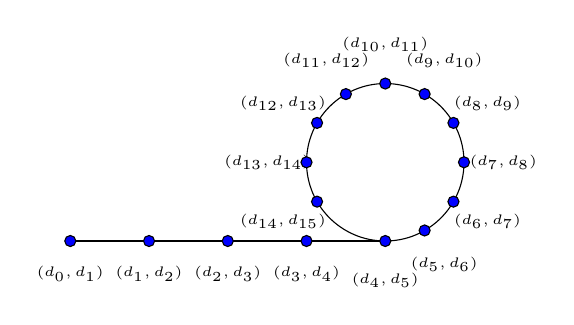
\begin{tikzpicture}
\draw (-4,-1) -- (0,-1);
\foreach[count=\i, evaluate=\i as \y using int(\i)] \x in {0,...,3}{
	\path[draw, fill=blue] (\x - 4,-1) circle[radius=2pt] node [below=2 mm] {\tiny{$(d_\x, d_\y)$}};
}
\draw circle [radius=1];
\foreach \a/\k/\h in {270/4/5, 300/5/6, 330/6/7, 0/7/8, 30/8/9, 60/9/10, 90/10/11, 120/11/12, 150/12/13, 180/13/14, 210/14/15}{
	  \draw  (\a: 1.5) node {\tiny{$(d_{\k},d_{\h})$}};	
      \path[draw, fill=blue]  (\a: 1) circle[radius=2pt];
}
\end{tikzpicture}
\caption{Periodic sequence of pairs preceded by a prefix of pairs.}
\label{fig:looppairs}
\end{marginfigure}

The sequence of ordered pairs $(d_n, d_{n+1})$ is periodic with a period $p$ of at most $10^6$. We can construct a lookup table holding values of $d_n$ from one period $p$ and then compute $d_n$ for large $n$ by going into the lookup table at $n \mod{p}$.

The periodic part of the sequence doesn't necessarily start with the first pair in the sequence or with the second or the third etc... There might be a sequence prefix of ordered pairs that don't repeat before it goes into the sequence loop of repeating pairs. 
{}
We write a function that computes the prefix and the period of the sequence using Floyd's cycle finding algorithm\footnote{Floyd's algorithm is described at \url{https://en.wikipedia.org/wiki/Cycle_detection\#Tortoise_and_hare}. We use the Haskell implementation from \url{https://wiki.haskell.org/Floyd's_cycle-finding_algorithm}}. 

Luckily it turns out that in this case the prefix is  $2, 6, 28$  and the periodic sequence has period $100$.

With the lookup table we can compute $d_n$ for any large $n$ in constant time. $d_n$ gives us the last three digits of $c_n$. Our goal though was to compute the last three digits before the decimal point of $a_n$.  

We know $c_n=\lceil a_n \rceil$, so $c_n - 1=\lfloor a_n \rfloor$. This means that to get the digits for $a_n$, we need to extract them from $d_n - 1$. Listing \ref{lst:last3digitshaskell} has the complete Haskell implementation.

\begin{fullwidth}

\lstinputlisting[language=Haskell, basicstyle=\small, label={lst:last3digitshaskell}, frame=trBL, caption={Haskell code to compute last 3 digits}]{Last3Digits.hs}

To check our computation we can use this Mathematica function:

\begin{mmaCell}[morepattern={n, n_Integer}]{Code}
  last3Digits[n_Integer] := Mod[IntegerPart[(3 + Sqrt[5])^n], 1000]
\end{mmaCell}

\end{fullwidth}
